\chapter{Cálculo de la constante $\mathcal{A}$ (Capítulo 2)} \label{apen:constante-A}

Como se menciona en el Capítulo \ref{cap:modelo} la temperatura en la pared, promediada en el tiempo y en la dirección $Z$, crece linealmente con la coordenada $x$, esto es, $\langle T_w \rangle = \mathcal{A} \hspace{0.5mm} x $. Se procede entonces con el cálculo de la constante $\mathcal{A}$. Esto se realiza mediante un balance de energía en el dominio de simulacion, es decir, $L_x \times L_y \times L_z$ (véase Figura \ref{fig:apendice-b}). 

\begin{figure}[H]
  \centering  
    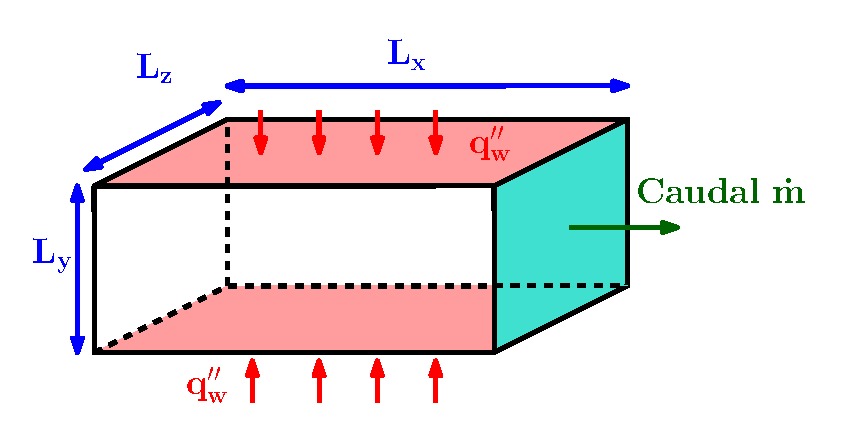
\includegraphics[width=0.6\textwidth]{figures/apendices/apendice_b.eps}
  \caption{Esquema del balance de energía.}
  \label{fig:apendice-b}
\end{figure}
De acuerdo a \cite{cengelheat}, dicho balance puede expresarse de la forma:
$$ q'' S = c_p \dot{m} \left( T_{out} - T_{in} \right)$$
donde $q''$ es el flujo externo de calor, $S$ es el área de sección transversal, $c_p$ es el calor específico a presión constante, $\dot{m}$ es el flujo másico, $T_{out}$ la temperatura del fluido a la salida ($x=L_x$) y $T_{in}$ la temperatura del fluido a la entrada ($x=0$). Considérese, por un lado, el cambio de variable realizado en la temperatura para satisfacer las condiciones de contorno períodicas (relaciones \ref{eq:pbc1} y \ref{eq:pbc2}), esto es, $T(x,y,z,t)= \langle T_w \rangle - \theta(x,y,z,t)$; y por el otro, que $T_{out}=T(x=L_x,y,z,t)$ y $T_{in}=T(x=0,y,z,t)$. Entonces, la diferencia de temperatura entre la entrada y la salida se puede escribir de la siguiente forma:

\begin{equation*}
\begin{aligned}
\left( T_{out} - T_{in} \right) &= T(x=L_x,y,z,t) - T(x=0,y,z,t) \\
								&= \left[ \mathcal{A} \hspace{0.5mm} L_x - \underbrace{\theta(x=L_x,y,z,t)}_{=0} \right] - \underbrace{ \left[ \mathcal{A} \hspace{0.5mm} 0 - \theta(x=0,y,z,t) \right] }_{=0} \\
								&= \mathcal{A} \hspace{0.5mm} L_x
\end{aligned}
\end{equation*}
Luego, si se tiene en cuenta que $q''= 2 q''_w$, $S=L_x L_z$ y se toma el flujo másico como la aproximación  $\dot{m} \simeq \rho_o \hspace{0.5mm} U_b \hspace{0.5mm} L_y \hspace{0.5mm} L_z $ (donde $U_b$ es la velocidad \textit{bulk} \cite{pope2001turbulent}), al juntar todo lo anterior se encuentra que 

$$ 2 q''_w  = c_p \hspace{0.5mm} \rho_o \hspace{0.5mm}  U_b \hspace{0.5mm} \mathcal{A}  \hspace{0.5mm} L_y \text{ .}$$ 
Finalmente, recordando que $L_y = 2 d$, donde $d$ es el semiancho del canal, se obtiene la expresión buscada:

\begin{equation}
\mathcal{A}=\frac{q''_w}{\rho_o \hspace{0.5mm} c_p \hspace{0.5mm} U_b \hspace{0.5mm} d } \text{ .}
\end{equation}








%
%``A efectos practicos las aproximacion de flujo de calor cte (condicion de Neuman) como una condición de Dirichlet igual a 0 resulta mejor desde el punto de vista numérico ya que la fluctuación de los campos es mayor y se requiere más tiempo de corrida para conseguir una buena estadistica ...''
%
%\begin{figure}[H]
%  \centering  
%  \subfloat[]{
%    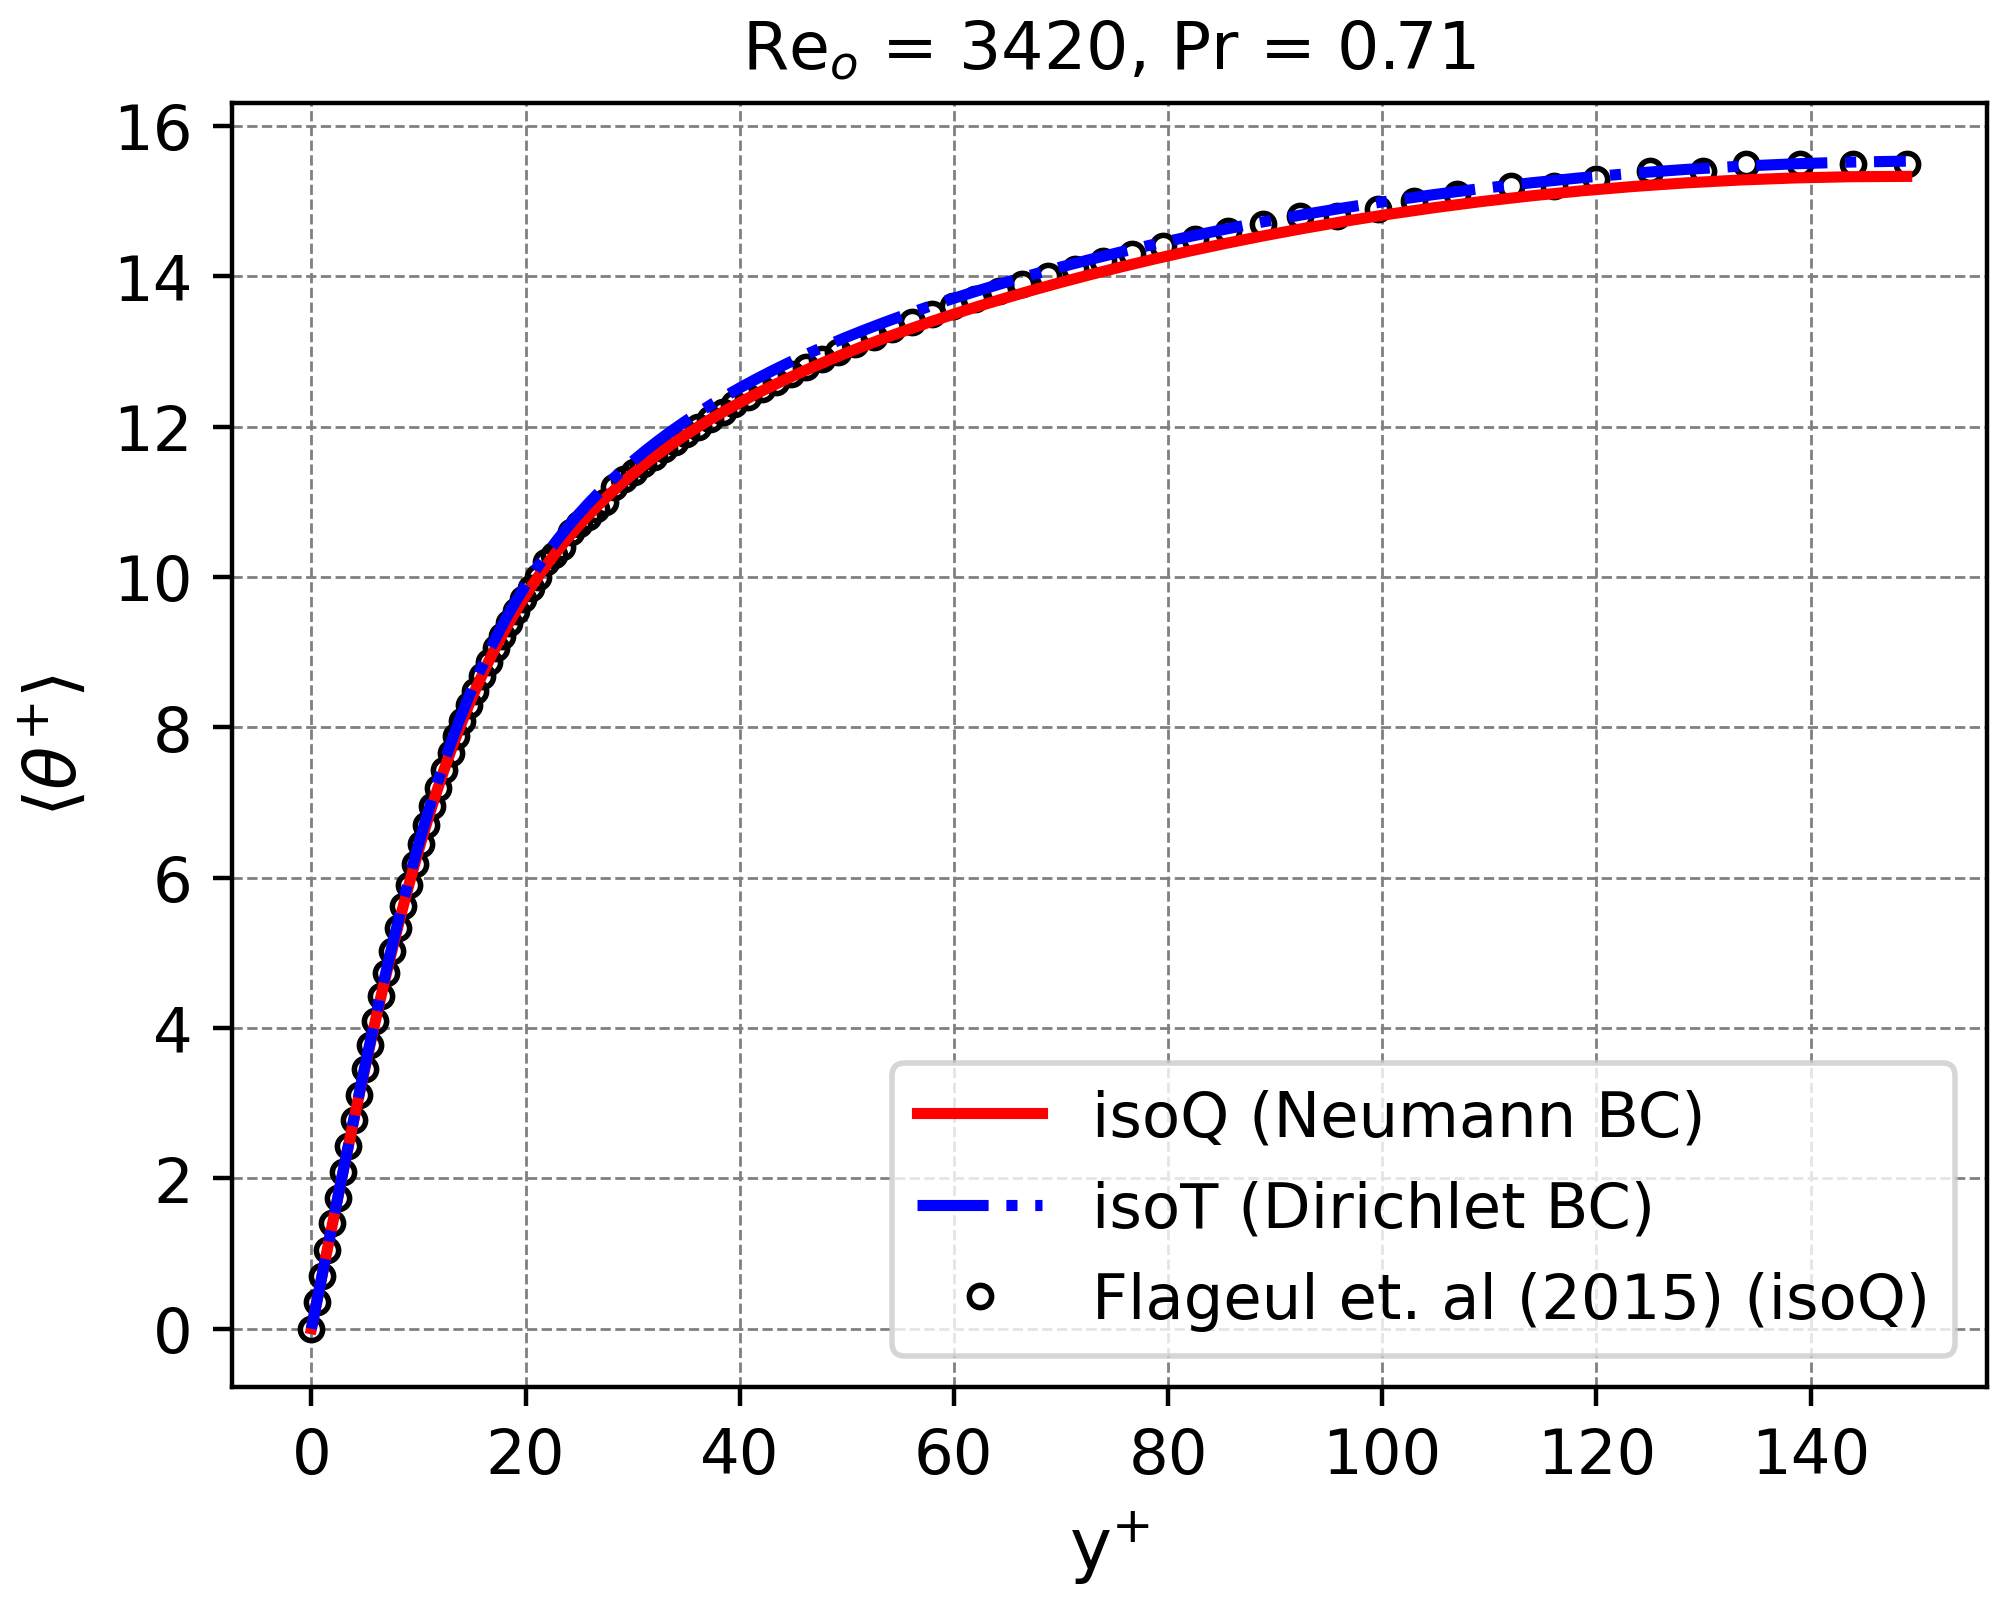
\includegraphics[width=0.49\textwidth]{figures/cap4/flageul/tep_theta.png}
%    \label{fig:flageul-theta}}
%  \subfloat[]{
%    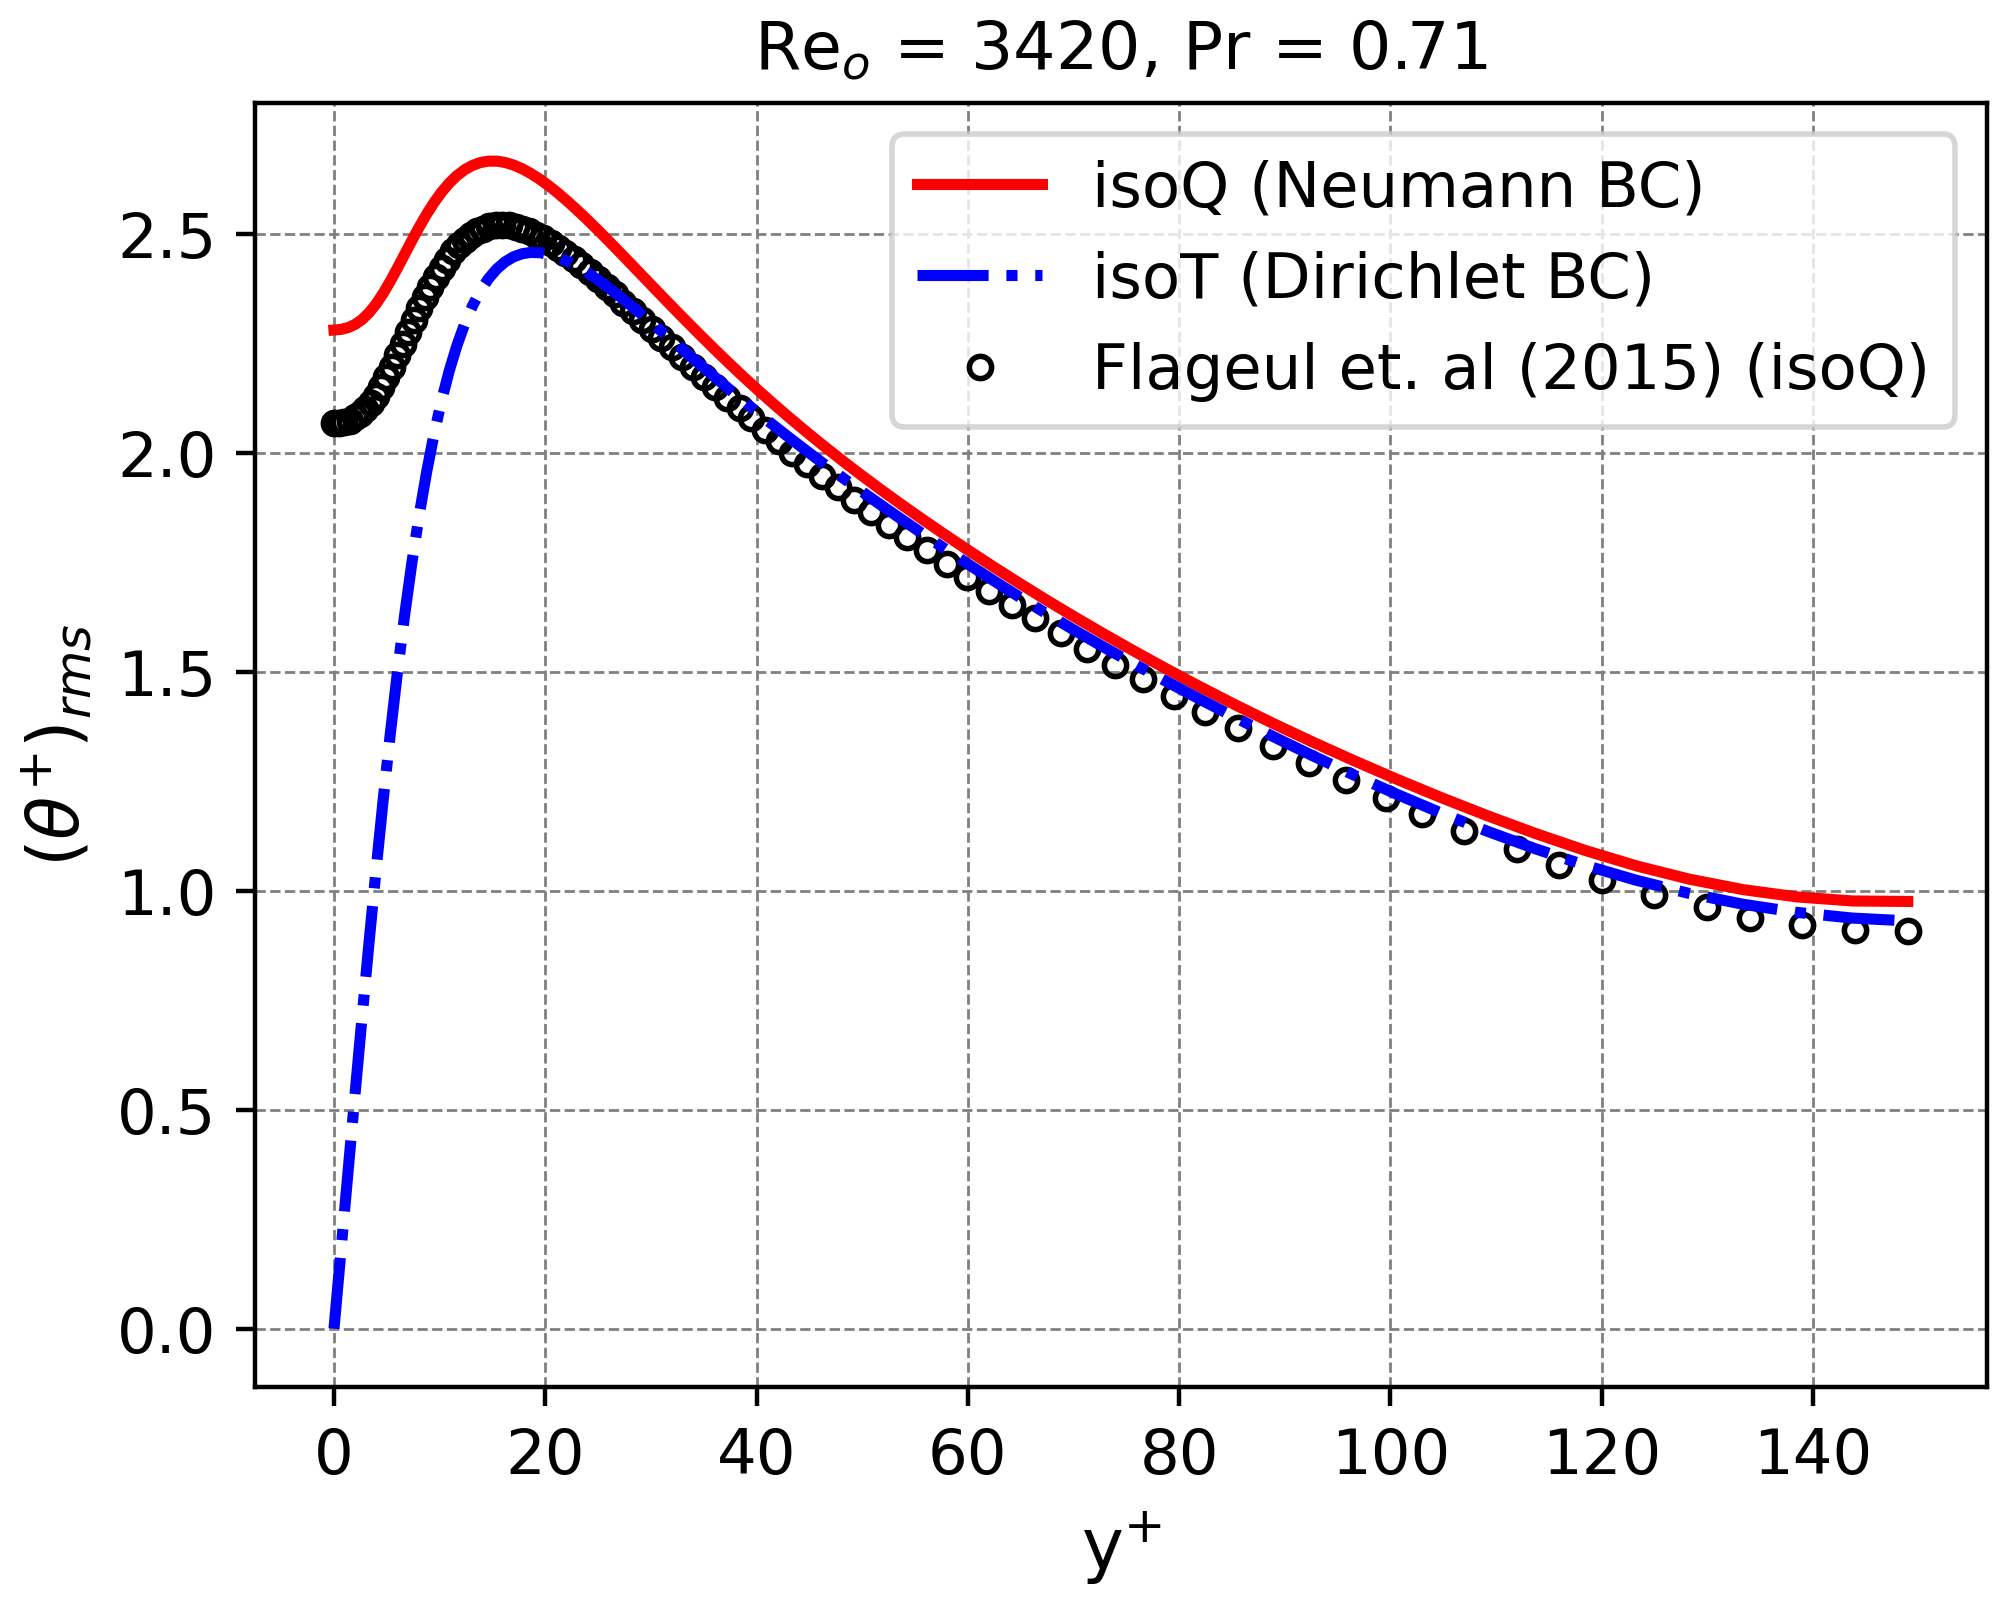
\includegraphics[width=0.49\textwidth]{figures/cap4/flageul/tep_thetap_rms.png}
%    \label{fig:flageul-theta-rms}}
%  \caption{}
%  \label{fig:flageul}
%\end{figure}
%
%\begin{figure}[H]
%  \centering  
%  \subfloat[]{
%    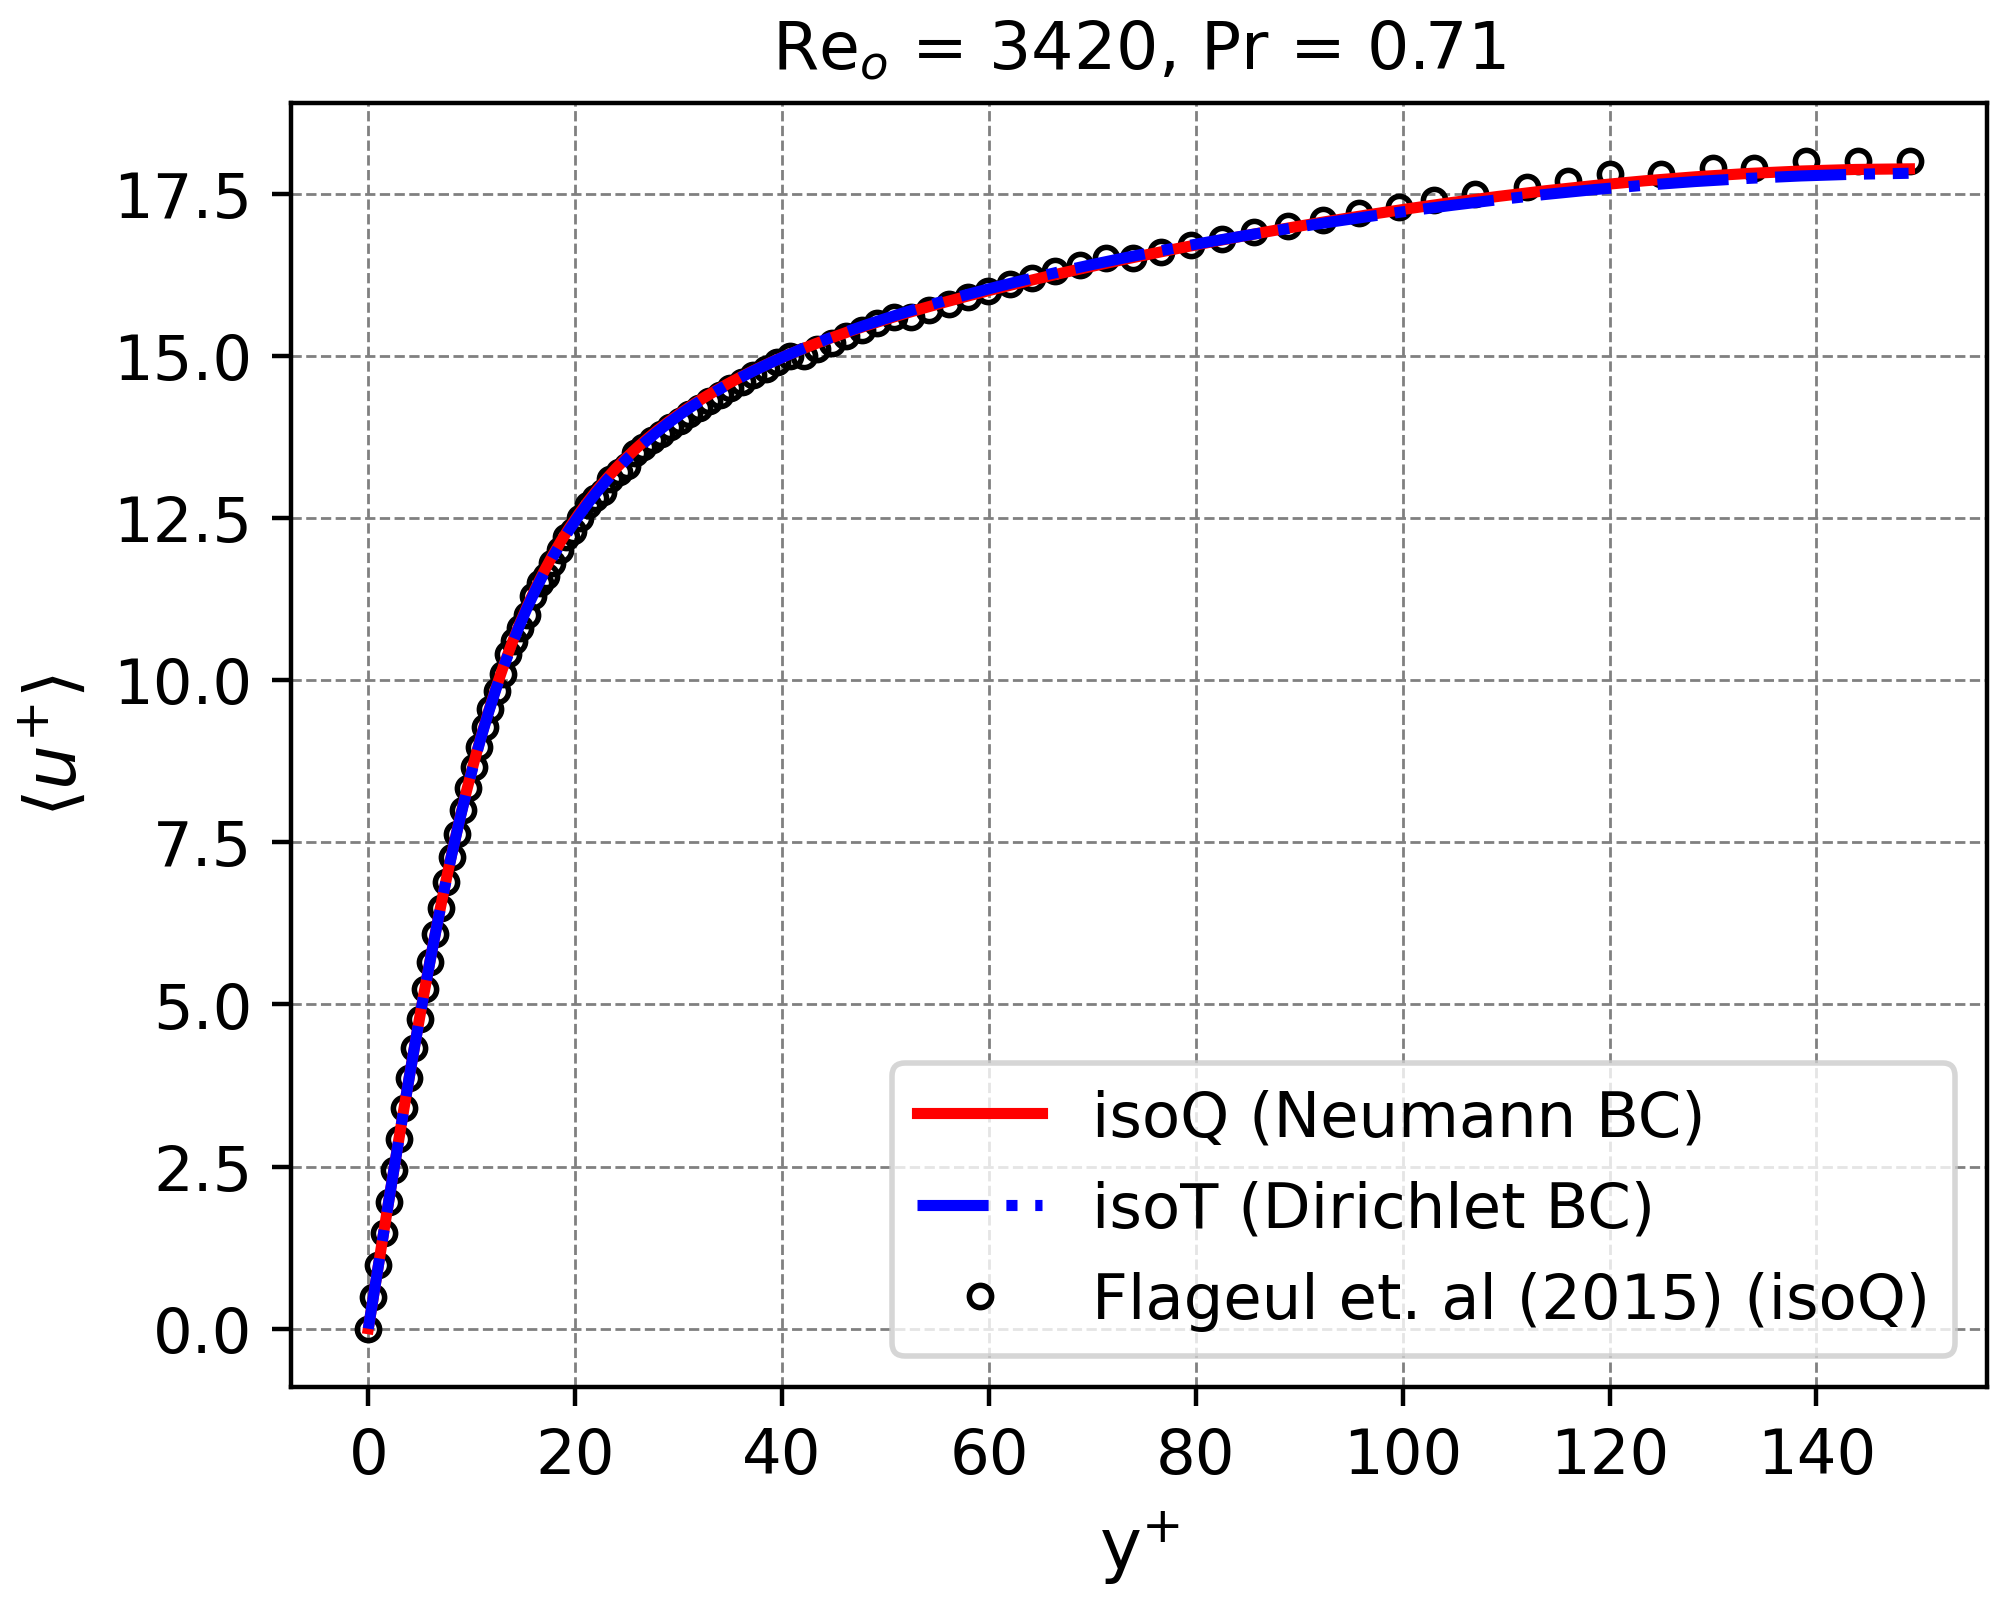
\includegraphics[width=0.49\textwidth]{figures/cap4/flageul/upmean.png}
%    \label{fig:flageul-up}}
%  \subfloat[]{
%    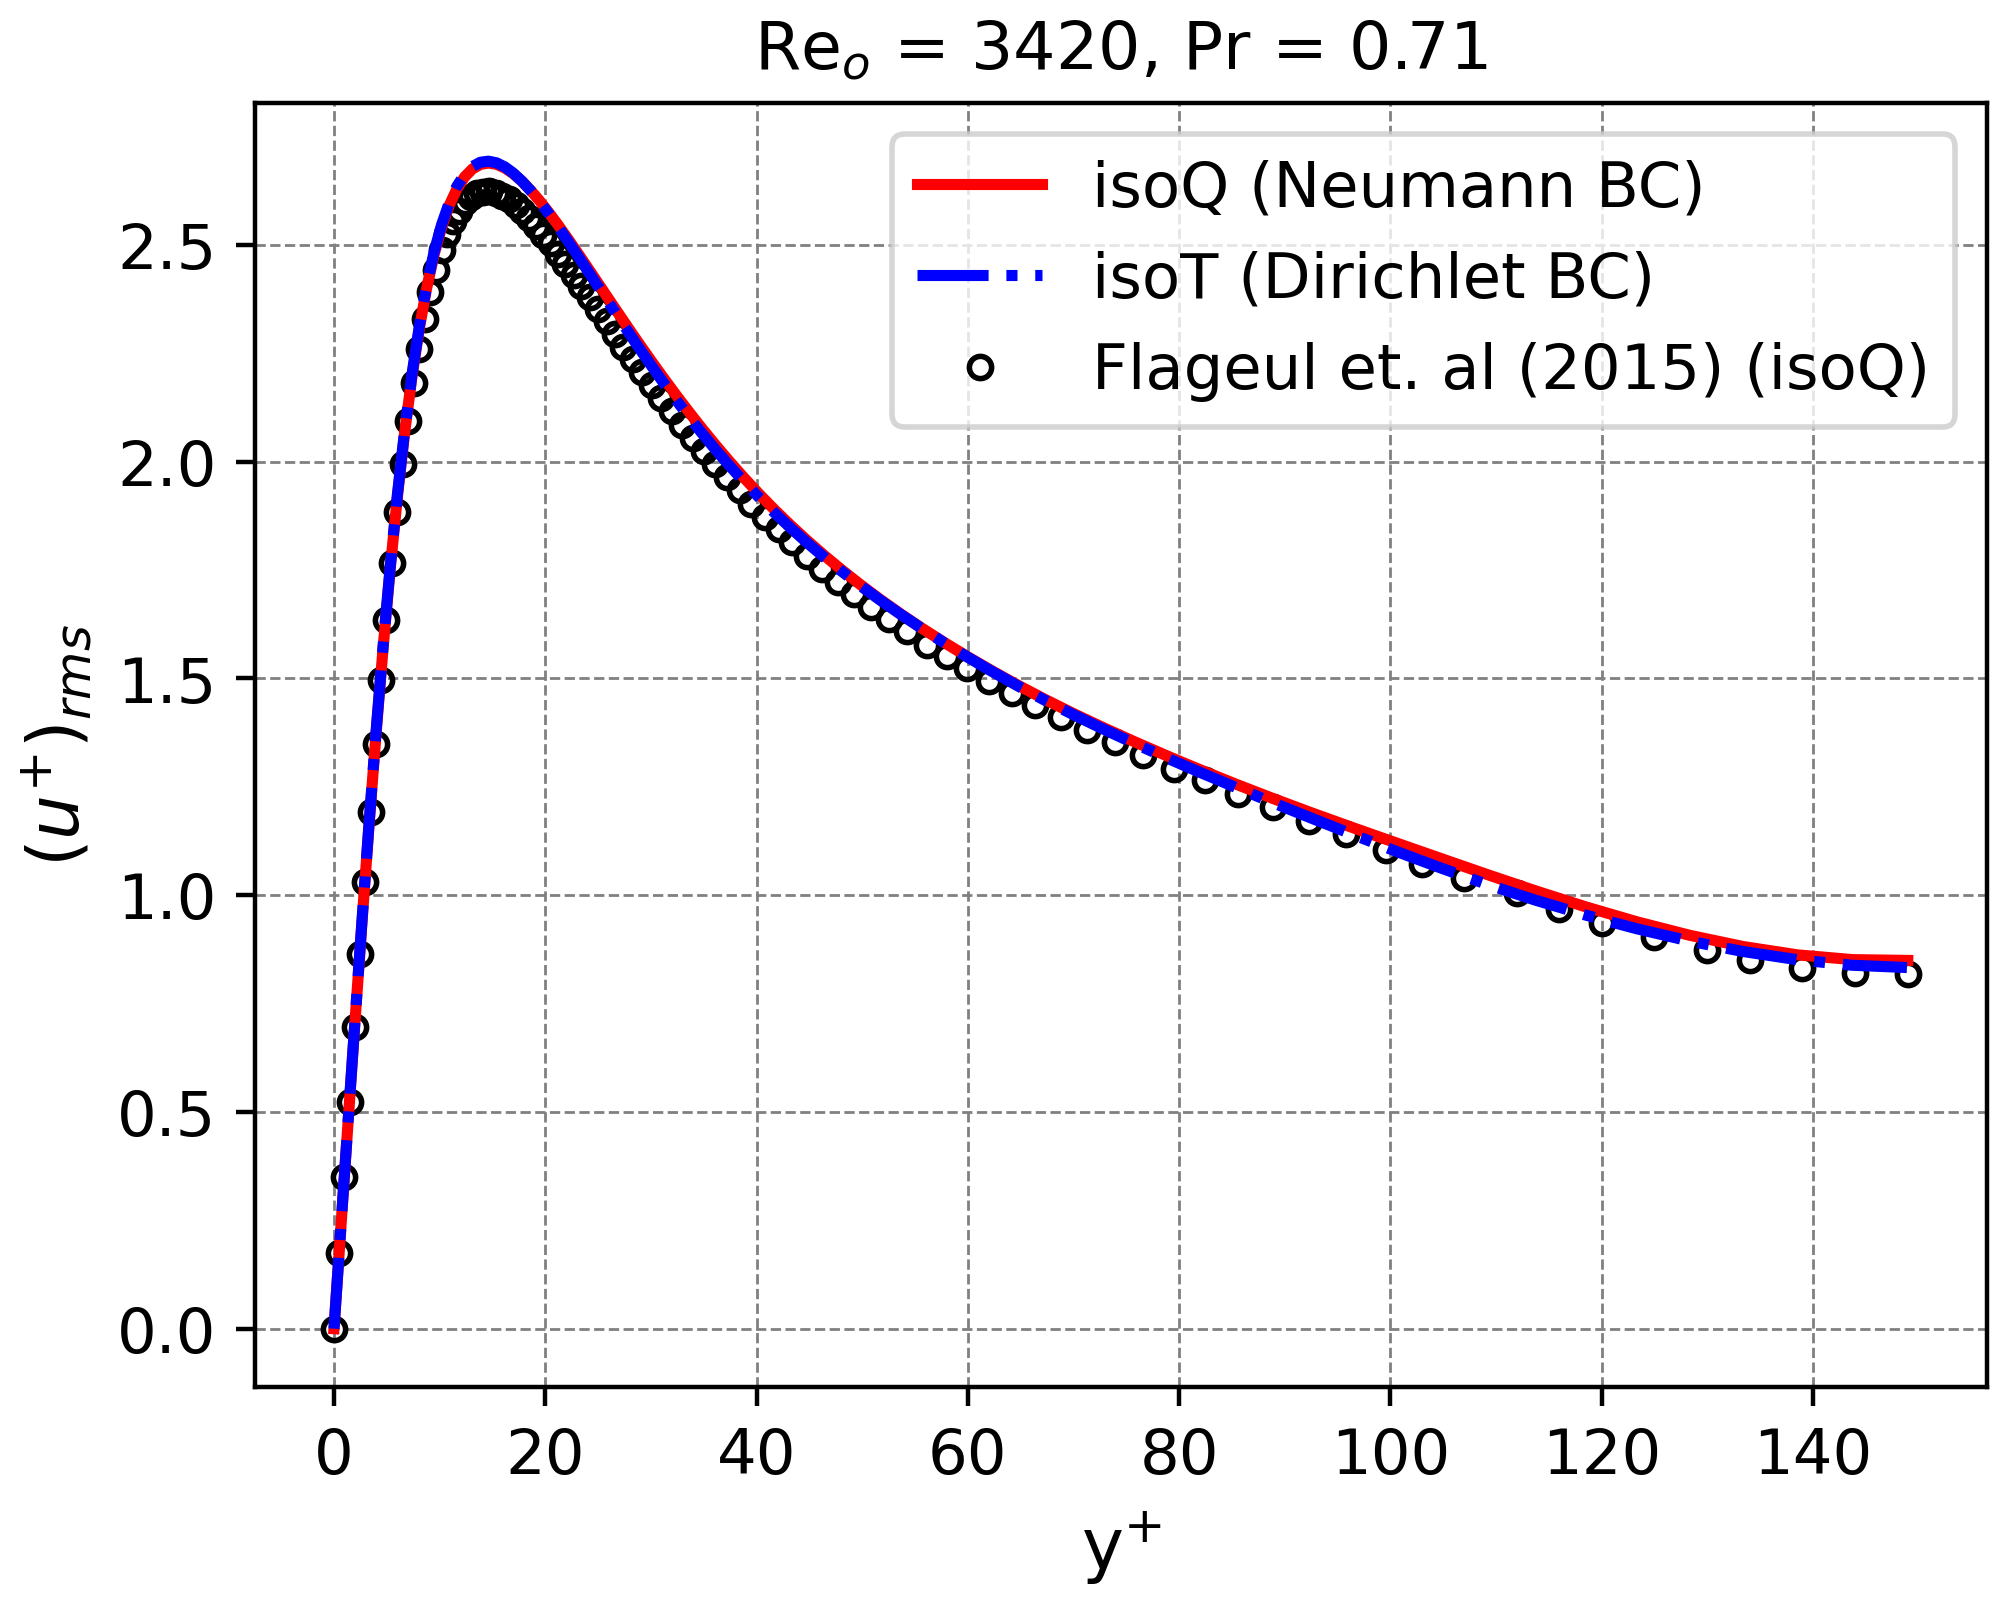
\includegraphics[width=0.49\textwidth]{figures/cap4/flageul/uprms.png}
%    \label{fig:flageul-up-rms}}
%  \caption{}
%  \label{fig:flageul}
%\end{figure}
%
%\begin{figure}[H]
%  \centering  
%    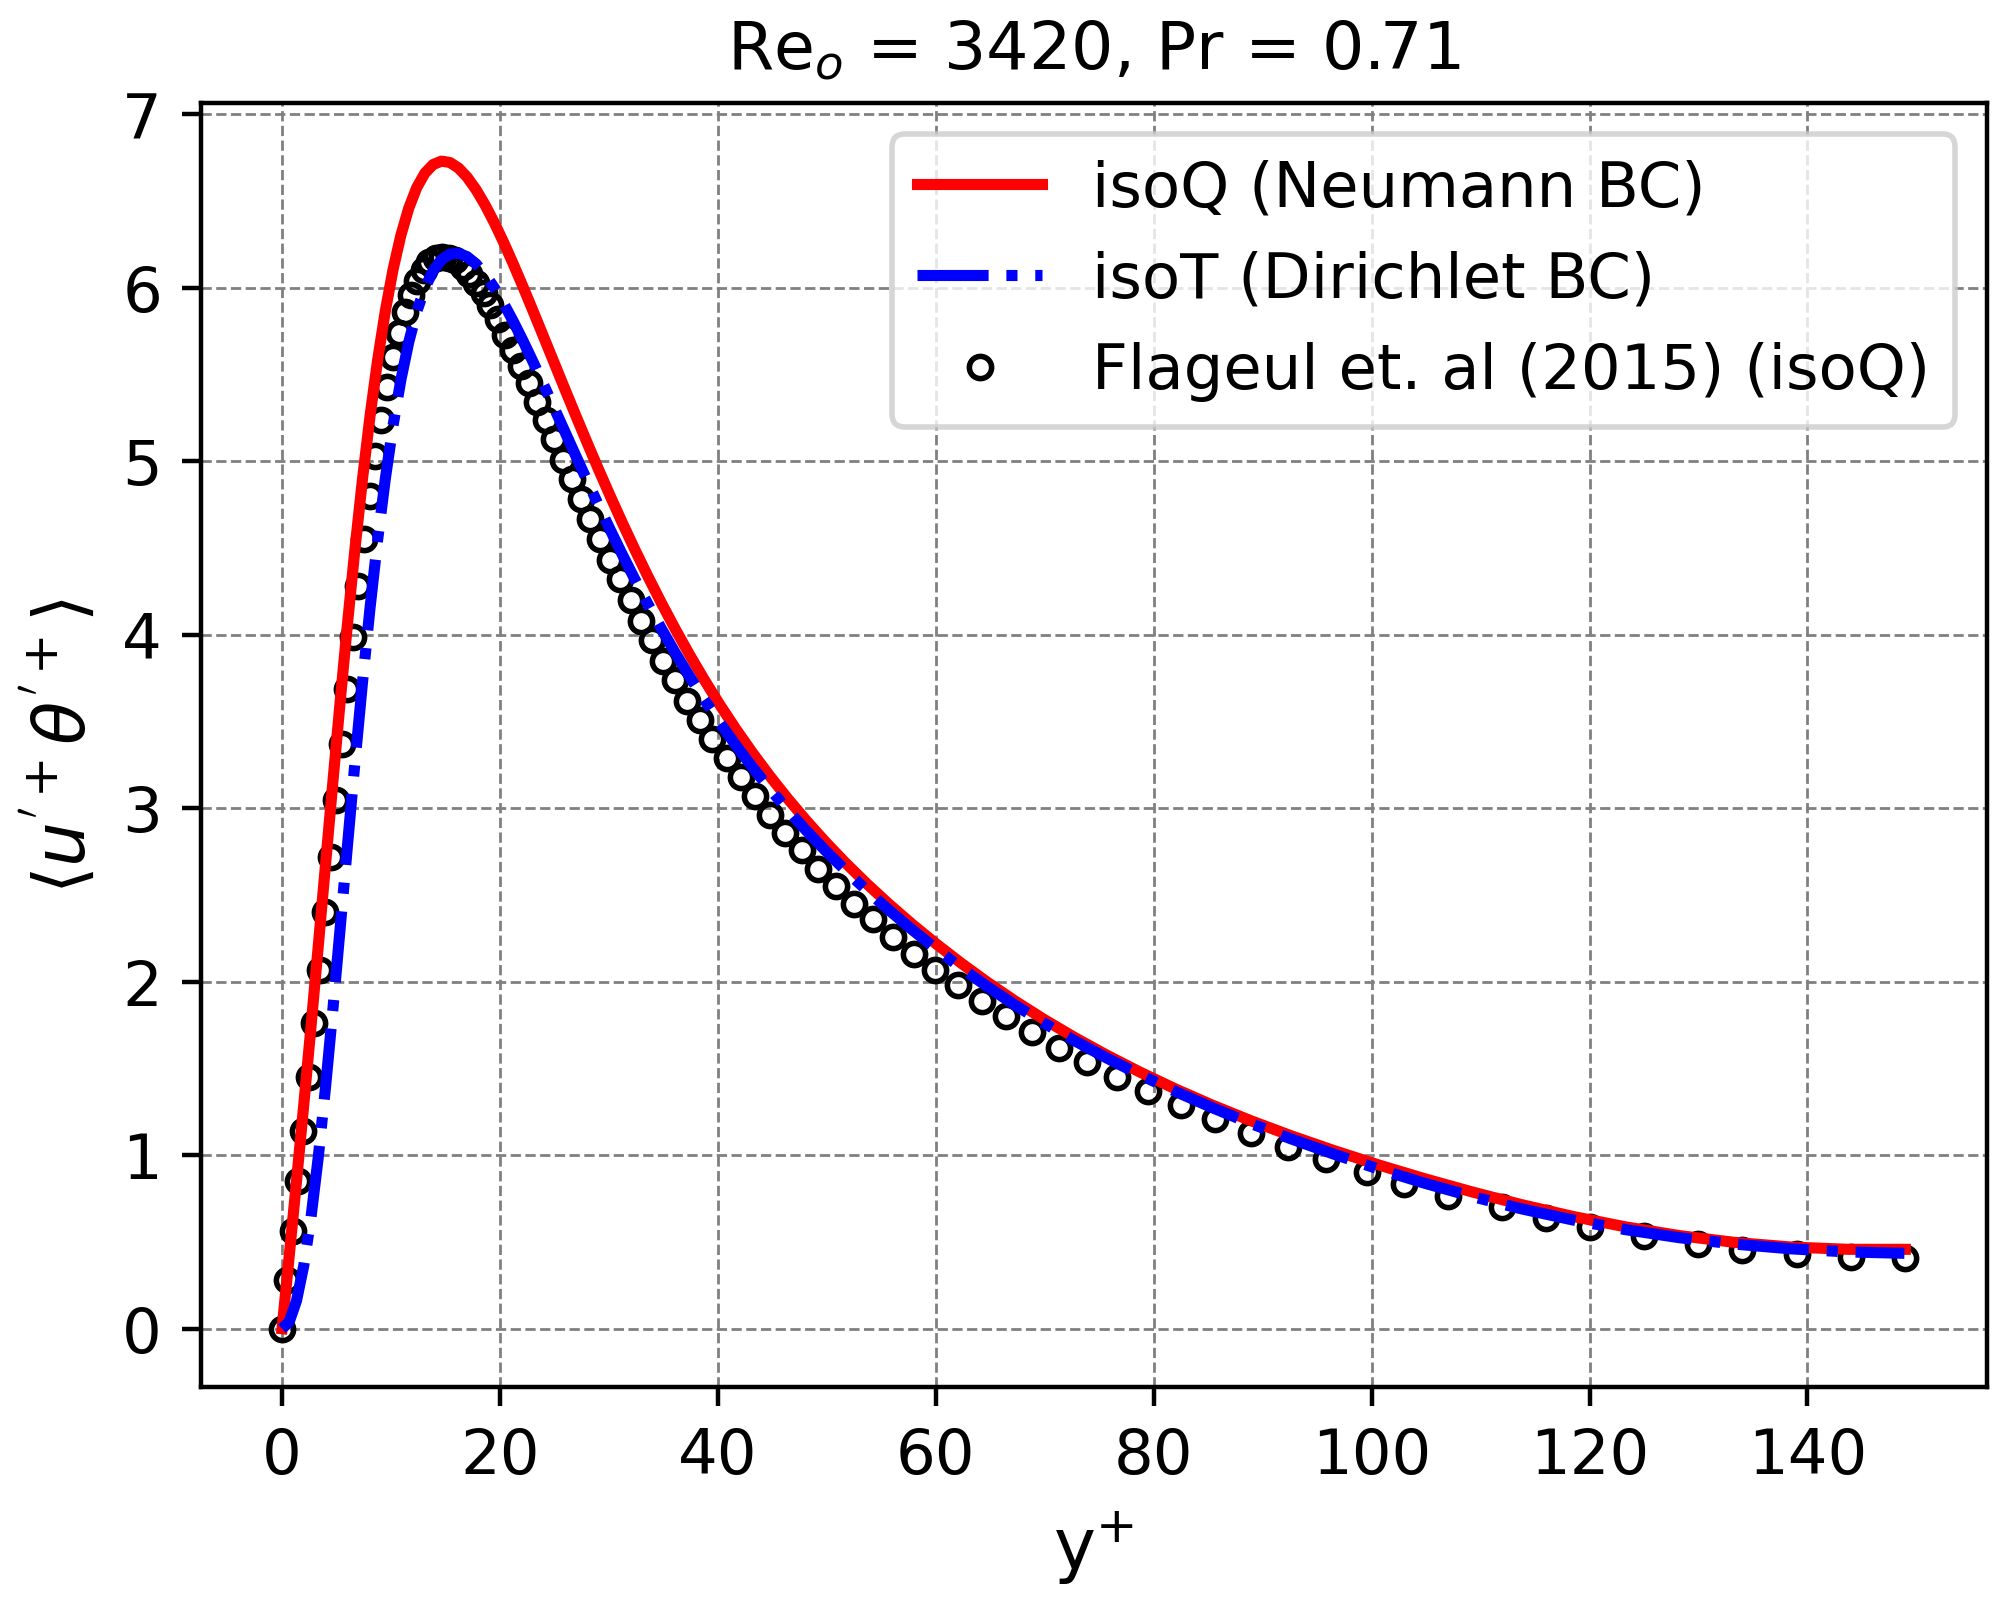
\includegraphics[width=0.49\textwidth]{figures/cap4/flageul/tep_up_thetap.png}
%    \label{fig:flageul-up-thetap}
%  \caption{}
%  \label{fig:flageul}
%\end{figure}

